\documentclass{DateStructure}

\SubjectName{车厢调度}
\CollegeName{理学院}
\Major{信息与计算科学}
\GroupNumber{第十六组}
\StudentA{20071226}{童繁}{进程图}
\StudentB{20071227}{王瀚功}{测试}
\StudentC{20071228}{王赛豪}{文案}
\StudentD{20071229}{吴政豪}{示意图}
\StudentE{20071230}{武琦}{代码}

\begin{document}	
\makecover
\newpage
\thispagestyle{empty}
\tableofcontents   
\newpage
\setcounter{page}{1} 
	
\section{需求分析}
\begin{itemize}
\item[(1)]设计一个程序,求出所有可能由车厢系列编号为1,2,...,n输出的长度为n的车厢序列;
\item[(2)]利用栈的顺序结构SqStack之上实现栈的基本操作,程序对栈的任何存取(即更改,读取和状态判别等操作)必须借助于基本操作进行;
\item[(3)]利用双向栈存储结构实现调度站和输出序列这两个栈的空间共享,并思考对于车厢序列长度n,两栈共享空间长度m;
\item[(4)]对于每个输出序列印出操作序列状态变化过程。
\end{itemize}

\section{概要设计}
一个数的进栈以后,有两种处理方式:要么立刻出栈,或者下一个数的进栈(如果还有下一个元素)。其出栈以后,也有两种处理方式:要么继续出栈(栈不为空),或者下一个数
的入栈。\par
要实现车厢调度,需要建立栈的顺序结构来实现栈的基本操作,并利用双向栈存储结构实现调度站和输出序列这两个栈的空间共享。最后,输出所有可能的序列并印出每个输出序列状态变化的过程。\par

\begin{figure}[H] 
\centering
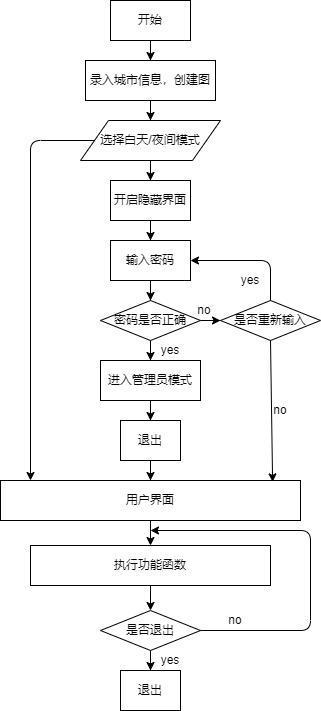
\includegraphics[width=300pt]{主函数.png}
\caption{主函数流程图}
\end{figure}

\section{详细设计}
\subsection{栈的表示与实现}
\subsubsection{栈的顺序存储表示}
\begin{lstlisting}[language=C,caption={栈的顺序存储}]
#define STACK_INIT_SIZE 100 //存储空间初始分配量
#define STACKINCREMENT 10 //存储空间分配增量
typedef int SElemType;
typedef int Status;
typedef struct
{
    SElemType *base;//栈底指针
    SElemType *top;//栈顶指针
    int stacksize;//栈容量
}SqStack;
\end{lstlisting}
\subsubsection{栈的基本操作函数}
\begin{lstlisting}[language=C,caption={栈的操作函数}]
Status InitStack(SqStack *S)//构造一个空栈S
{
    S->base=(SElemType *)malloc(STACK_INIT_SIZE*sizeof(SElemType));
    if(!S->base)
        exit(OVERFLOW);//存储分配失败
    S->top=S->base;
    S->stacksize=STACK_INIT_SIZE;
    return OK;
}

Status ClearStack(SqStack *S)//把S置为空栈
{
	S->top=S->base;
	return ERROR;
}

Status StackEmpty(SqStack *S)//若S为空栈,则返回OK;否则返回ERROR
{
	if(S->base==S->top)
		return OK;
	else
		return ERROR;		
}

SElemType StackLength(SqStack *S)//返回S的元素个数,即栈的长度
{
	return S->top-S->base;
}

Status Push(SqStack *S,SElemType e)//插入元素e为新的栈顶元素
{
	if(S->top-S->base>=S->stacksize)//栈满,追加存储空间
	{
		S->base=(SElemType *)realloc(S->base,(S->stacksize+STACKINCREMENT)*sizeof(SElemType));
		if(S->base)
			exit(OVERFLOW);//存储分配失败
		S->top=S->base+S->stacksize;
		S->stacksize+=STACKINCREMENT;	 
	}
	*(S->top++)=e;
	return OK;
}

Status Pop(SqStack *S,SElemType *e)//若栈不空,则删除S的栈顶元素,用e返回其值,并返回OK;否则返回ERROR
{
    if(S->top==S->base)
        return ERROR;
    *e=*(--S->top);
    return OK;
}
\end{lstlisting}
\subsection{双栈实现车厢调度}
\begin{figure}[H] 
\centering
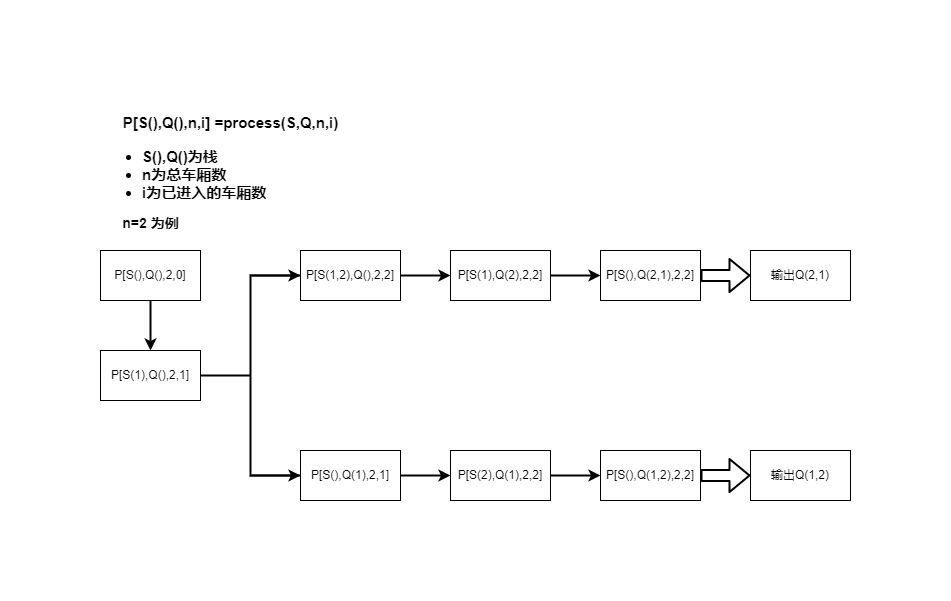
\includegraphics[width=500pt]{process.png}
\caption{Process函数示意图}
\end{figure}
\begin{lstlisting}[language=C,caption={车厢调度函数}]
Status Process(SqStack *S,SqStack *Q,SElemType n,SElemType i)
{
    //找出当前元素进栈后所有可能的操作
    SElemType *e,a;
    e=&a;
    if(i<n)//编号进栈递归 
    {
        Push(S,i+1);
        Process(S,Q,n,i+1);
        Pop(S,e);
        i--;
    }
    if(!StackEmpty(S))//递归处理出栈
    {
        Pop(S,e);
        Push(Q,a);
        Process(S,Q,n,i+1);
        Pop(Q,e);
        Push(S,a);
    }
    if(StackLength(Q)==n&&StackEmpty(S))//输出可能的方案
    {
        printf("第%d种情况:",t);
        Print(Q);
        t++;
    }
}
\end{lstlisting}
\subsection{车厢序列及其状态变化过程的输出}
\begin{lstlisting}[language=C,caption={打印函数}]
Status Print(SqStack *S)//打印序列状态变化过程
{
    SElemType *p,i,max=0;
	p=S->base;
	while(p!=S->top)//输出序列
	{
		printf("%d",*p);
		p++;
	}
    printf("  具体过程:");
    p=S->base;
    while(p!=S->top)//输出序列状态变化过程
	{
        for(i=max+1;i<=*p;i++)
            printf("%d进 ",i);
        printf("%d出 ",*p);
        if(max<*p)
            max=*p;
		p++;
	}
	printf("\n");
}
\end{lstlisting}	
\begin{figure}[H] 
\centering
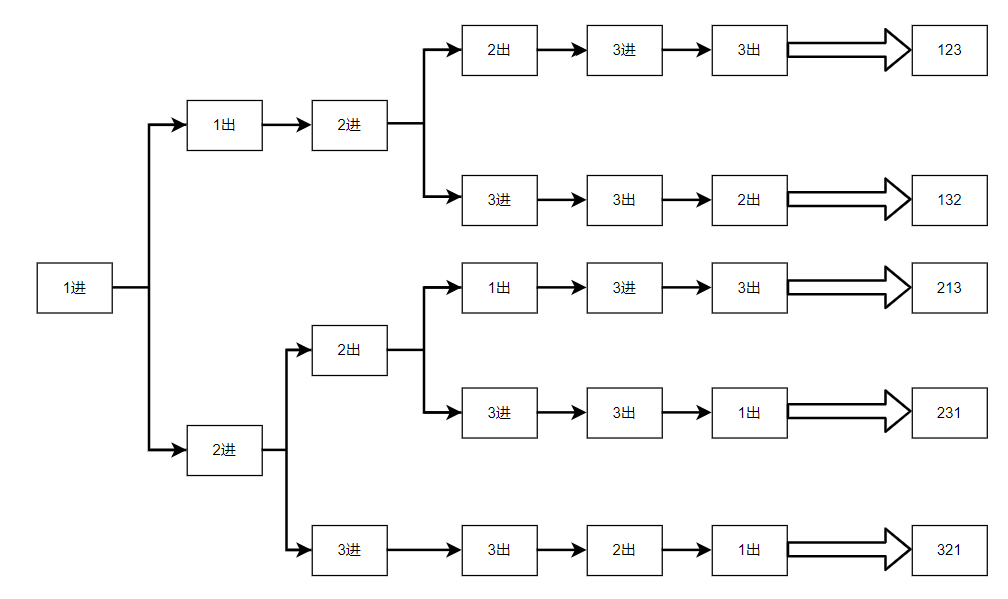
\includegraphics[width=400pt]{序列状态变化.png}
\caption{n=3时的序列变化情况}
\end{figure}

\section{功能测试}
分别取n=1,2,3和4,测试程序:\par
\begin{figure}[H] 
\centering
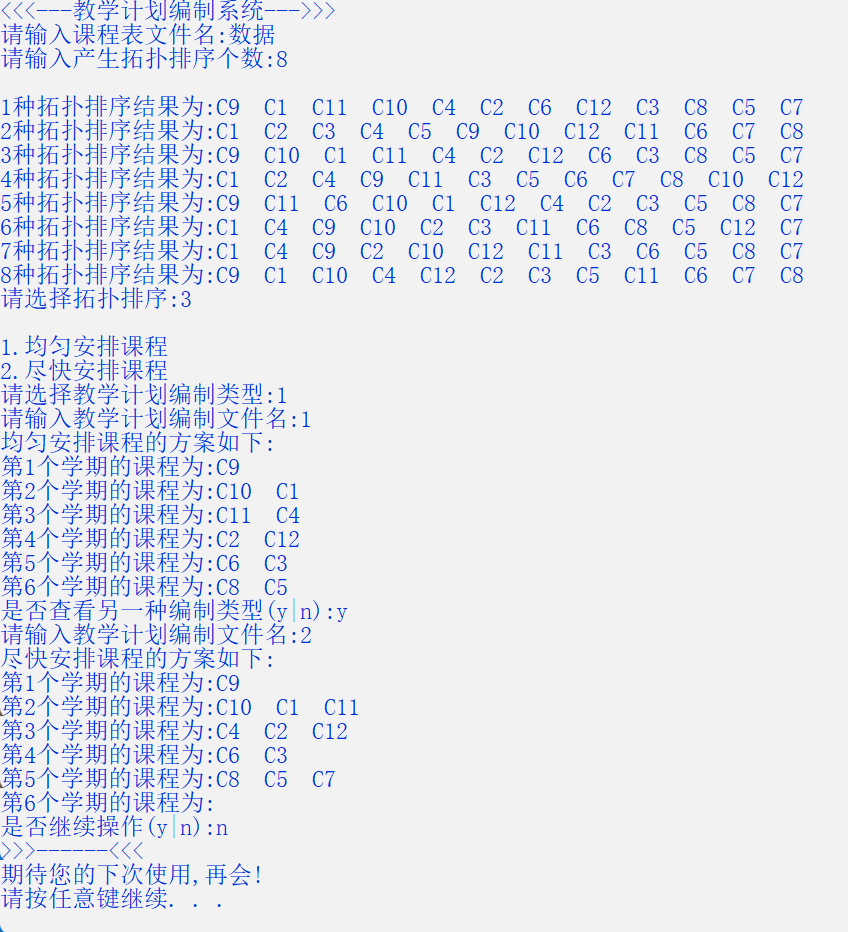
\includegraphics[width=400pt]{测试.png}
\caption{功能测试}
\end{figure}

\section{研究思考}
对于车厢序列长度n,两栈共享空间长度m取n最合适。理由如下:\par
1.m<n\par
当双栈存入m个数据时,s.top2-s.top1=1(满栈),无法存入n个数据。\par
\begin{figure}[H] 
\centering
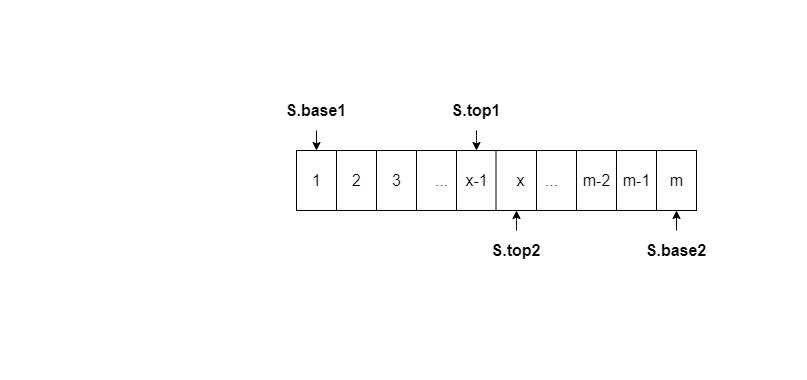
\includegraphics[width=400pt]{m1.png}
\caption{m<n时}
\end{figure}
2.m=n\par
当双栈存入n个数据时,s.top2-s.top1=1(满栈),刚好存入n个数据。\par
\begin{figure}[H] 
\centering
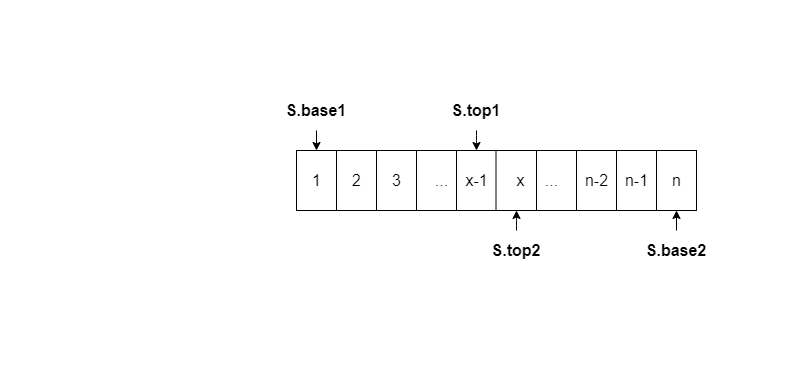
\includegraphics[width=400pt]{m2.png}
\caption{m=n时}
\end{figure}
3.m<n\par
当双栈存入n个数据时,s.top2-s.top1>1(满栈),足够存入n个数据。\par
\begin{figure}[H] 
\centering
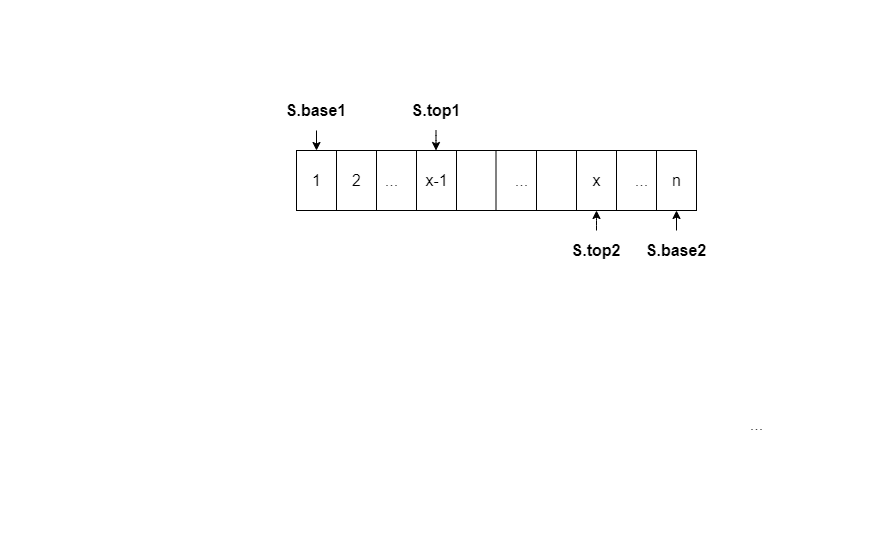
\includegraphics[width=400pt]{m3.png}
\caption{m>n时}
\end{figure}
故综上:m=n时能刚好处理n个数据,并且所用空间最小。\par

\section{心得体会}
这次课程设计的心得体会通过实践我们的收获如下:\par
1、巩固和加深了对数据结构的理解,提高了综合运用本课程所学知识的能力。\par
2、培养了独立思考,深入研究,分析问题、解决问题的能力。\par
3、通过实际编译系统的分析设计、编程调试,掌握了应用软件的分析方法和工程设计方法。\par
总的来说,这次课程设计让我们组获益匪浅,对数据结构也有了进一步的理解和认识。\par

\newpage 
\section{附录}
\lstinputlisting[language=C]{main.c}
\end{document}
